%\documentclass[12pt,letterpaper,final]{article}
\documentclass[12pt,letterpaper,final]{article}
\usepackage[latin1]{inputenc}
\usepackage{amsmath}
\usepackage{amsfonts}
\usepackage{amssymb}
\usepackage{graphicx}
\usepackage{fullpage}
\usepackage{cite}
\author{H.S. Barnard}
\title{Preliminary Design Report: Electron beam EDX analysis for magnetic fusion devices}
\begin{document}
\maketitle
%\abstract{Abstract Abstract Abstract Abstract Abstract }
%

\section{Introduction}

Plasma material interactions (PMI) is a critical area of study for magnetic fusion devices.  Understanding the effects of PMI including erosion, deposition, fuel retention, and impurity production all play a vital role in the development of fusion reactors. The successful demonstration of the accelerator-based in-situ materials surveillance (AIMS) diagnostic clearly shows that particle beam based in-situ diagnostics can provide measurements of the effects of PMI with unprecedented spatial and temporal resolution \cite{barnard2014thesis,hartwig2013thesis,hartwig2013situ}.

AIMS is essentially an in-situ implementation of ion beam analysis (IBA) techniques that are commonly used for materials analysis. The IBA used in AIMS is similar to particle induced gamma emission (PIGE) and nuclear reaction analysis (NRA) for low-Z elements. Performing spatially resolved analysis in-situ requires steering the beam using the tokamaks magnetic fields.  This adds additional engineering challenges, but provides PMI analysis capabilities over unprecedented time-scales and spatial scales. The current application of AIMS is effective for isotopic measurements of low-Z materials \cite{hartwig2014fuel,barnard2015boron}. To expand on this capability, a similar technique using an electron beam can be used for in-situ analysis to provide a complementary set of measurements. The electron beam analysis is similar to energy dispersive X-ray spectroscopy (EDX or EDS) -- is commonly used in electron microscopy -- and can be used to make quantitative measurements the elemental composition of most elements with the exception of hydrogen and helium \cite{goldstein1997scanning}. 

In Alcator C-Mod and other tokamaks, there are many PMI effects that can be studied EDX. Effects like plasma erosion and deposition and material migration can all be studied with in-situ EDX analysis. For example, changes in thickness of surface layers can be measured directly. Erosion and deposition of bulk wall material can be measured with implanted depth markers. Furthermore, the overlap in beam physics, detection techniques, and established electron microscopy techniques will allow the development of in-situ EDX in tokamaks to draw from the development of AIMS and decades of EDX experience in the microscopy.

\section{Energy dispersive X-ray analysis in a tokamak}

The goal of tokamak EDX is to provide macroscopic EDX measurements with $\sim1$~cm spot size over the entire poloidal range of the tokamak wall and over significant fraction of the toroidal range. This can be done using an electron beam (section \ref{sec:ElectronGun}) which scanned over the wall of the tokamak using the tokamak's magnetic field coils (section~\ref{sec:BeamSteering}) to induce X-rays in the material surface (section~\ref{sec:BeamInteractions}). Spectroscopic analysis of these X-rays is performed with silicon drift detectors (section~\ref{sec:detectors}) to provide quantitative analysis of the elemental composition of the surface. 

When EDX is used in microscopy there is relatively small variation in detection geometry throughout the spatial range of measurements due to the small beam deflections (nm-$\mu$m scale). For tokamak EDX however, the macroscopic (cm-m scale) dimensions of the measurements make modeling of the beam and detector geometry challenging. With the experience and simulation tools developed for the AIMS diagnostic, tokamak EDX can be achieved using modern electron beam and X-ray detection technology.

\subsection{Beam steering and modeling}
\label{sec:BeamSteering}
Like AIMS, the tokamak's magnetic fields are used to steer the electron beam to target PFCs for analysis. Compared to a $\sim 1$~MeV ion beam, the magnetic field required to steer an electron beam with energy in the relevant range for EDX (10-100~keV) along an identical trajectory is substantially less. This can be seen by comparing the magnetic rigidity $R$ for a beam used for AIMS to an electron beam (shown in figure \ref{fig:Rigidity}). Magnetic rigidity is defined as $B\rho = R(m_o,T)$, providing the relationship between the radius of curvature $\rho$, the applied magnetic field $B$, and the beam's rest mass $m_o$ and kinetic energy $T$. This is useful for comparison because for a given trajectory, the required magnetic field is directly proportional to $R(m_o,T)$. \textbf{... More on beam simulation...}.

\begin{figure}[!h]
 \centering
  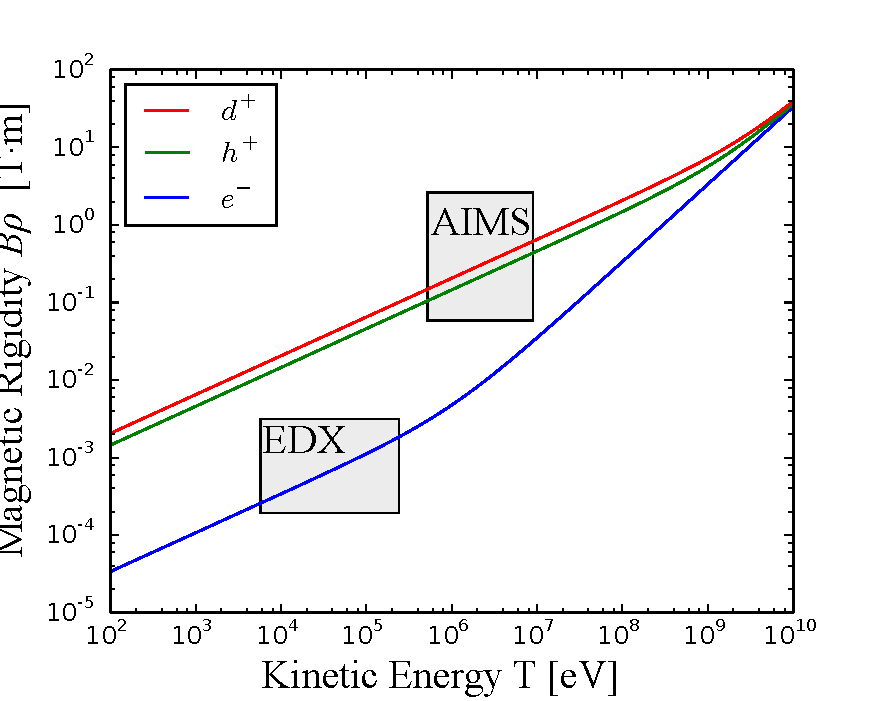
\includegraphics[width=\columnwidth]{figures/MagneticRigidity.pdf}
 \caption{Magnetic rigidity is shown versus kinetic energy for ion beams and electron beams. Magnetic rigidity $R$ relates radius of curvature $\rho$ and the applied magnetic field $B$ such that $B\rho = R(E)$. The shaded areas indicate the operating energy range for EDX and AIMS.}
 \label{fig:Rigidity}
\end{figure}

\section{Beam interactions with materials}
\label{sec:BeamInteractions}
Electron beams interacting with matter are more complicated than ion beams. Ion beams are relatively simple to model because the ions lose energy approximately monotonically with distance with minimal straggling. Electron beams, however, interact primarily through large-angle scattering and undergo many scattering, atomic excitation, and ionization events before either coming to rest or exiting the material surface. As a result, Monte Carlo methods are often used to study electron beams to predict the energy and spatial distribution of the electron trajectories as well as the X-ray emission. Analysis was performed for this study using CASINO 2.48 \cite{CASINO} and MC X-Ray Lite \cite{MCXRayLite}, both simulation packages developed for electron microscopy and EDX. The complexity of the of the electron scattering can be seen from figure~\ref{fig:ElectronsInTarget}.

\begin{figure}[!h]
 \centering
  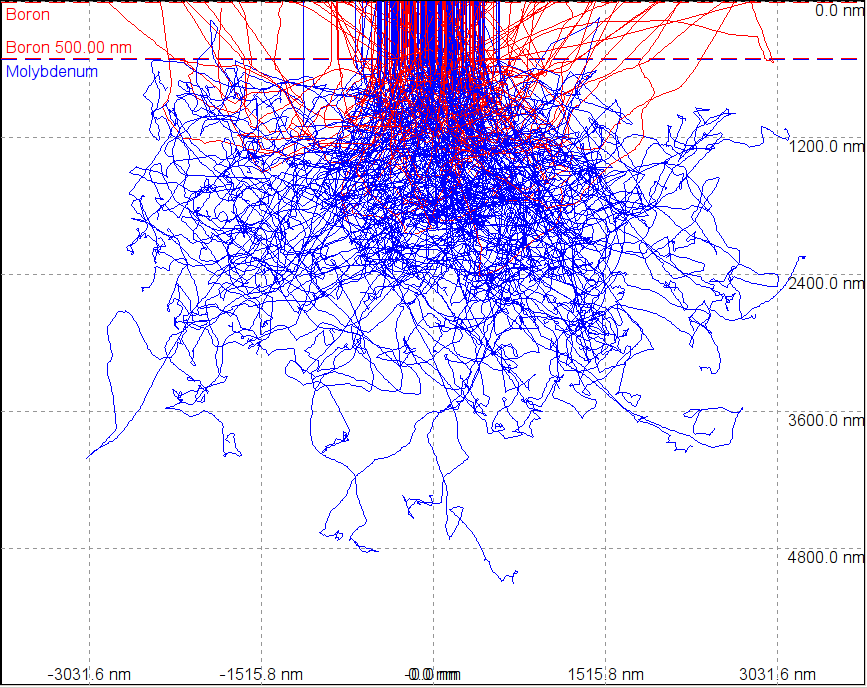
\includegraphics[width=\columnwidth]{figures/ElectronsInTargetWide.png}
 \caption{Monte Carlo simulation of electrons interacting with a boron coated molybdenum target, generated with CASINO 2.48 \cite{CASINO}. A 1~$\mu$m diameter beam is shown to keep the beam size comparable to the scattering length scales within the target. Red trajectories represent electrons that backscatter and exit the material surface. Blue trajectories represent electrons that come to rest within the material.}
\label{fig:ElectronsInTarget}
\end{figure}

\subsection{X-Ray excitation with electron beams}

For materials analysis, X-rays from K and L shell transitions are commonly used. These X-rays result from the transitions following inner shell ($n=1$) and second shell ($n=2$) ionization respectively. These X-rays are typically $\sim 0.1 - 100$~keV and are produced at distinct characteristic energies that are unique to each element. Since each element has a distinc atomic structure, and therefore distinct emission spectra, spectroscopic analysis of these X-rays can, in principle, be used to directly measure the elemental composition of the material.

The process of X-ray production from electron bombardment involves several effects that complicate the analysis. The K and L ionization cross sections are dependent on electron energy. X-ray emission resulting from these ionization events also competes with other de-excitation processes, such as Auger electron emission. In addition, the X-rays are attenuated as they exit the material. Furthermore, electrons undergo multiple large angle scattering events with a significant fraction leaving the surface before coming to rest which means that the interaction cross sections must be applied to each electron rather than beam as a whole. These effects can complicate the analysis but are readily accounted for in the MC simulation.% The main consequence is for the measurement is that Auger electrons must be obstructed or deflected so they do not interfere with the detector.

\subsection{Backscattered Electrons}

As electrons from the beam penetrate the material and substantial fraction of them backscatter out of the material surface after one or more collisions.  This is seen in the backscattered electron energy spectrum shown in figure~\ref{fig:BackscatteringSpectrum}. Backscattering is important to consider because 1) X-ray detectors are sensitive to electrons as well as photons, and 2) many of the electrons that leave the surface have sufficient energy to produce X-rays elsewhere in the within the vessel.

\begin{figure}[!h]
 \centering
  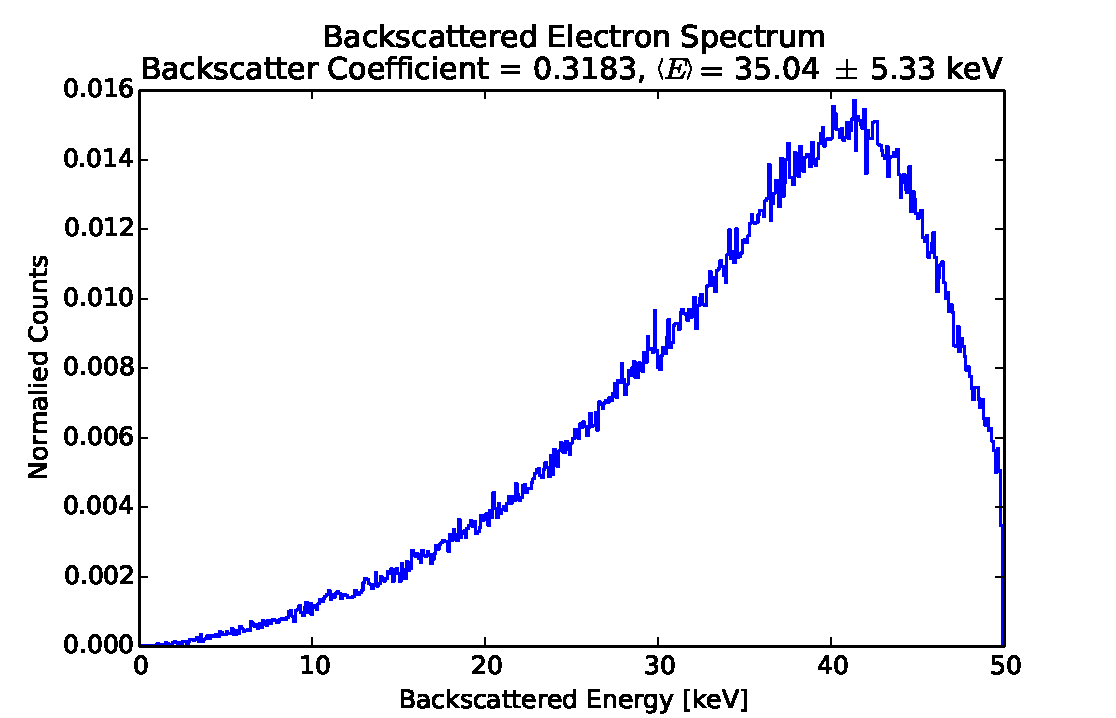
\includegraphics[width=\columnwidth]{figures/MolybdenumBackscatteringSpectrum.pdf}
 \caption{Electron backscattering spectrum for 50~keV electrons with normal incidence on molybdenum. (NOT NECESSARY FOR PAPER)} 
 \label{fig:BackscatteringSpectrum}
\end{figure}

For 50~keV electrons scattering off of molybdenum the backscattering coefficient is $\approx 0.3$ (fraction of beam electrons that backscattered) for normal incidence and tends to increase with incident angle.  For this case the mean backscattered energy of 35~keV which is sufficient to produce X-rays when these electrons interact with other surfaces. In order to make spatially resolved EDX measurements, it is therefore necessary to shield the detector from X-rays resulting from backscattering. Methods of shielding these X-rays and electrons from the detector are described in section~\ref{sec:DetectionGeometry}.

\section{Tokamak EDX Hardware}

A tokamak EDX can be implemented with presently available technology.  However, the technique poses some engineering challenges that must be addressed. This section provides an overview of the hardware that will be necessary with discussion of the engineering that is involved.

\subsection{Electron beam accelerator}
\label{sec:ElectronGun}

Electron beams have been studied and used for nearly a century for many applications in science and industry. As a result, electron accelerators or electron `guns' are a highly refined, mature, commercially available technology and can be built with beam parameters spanning the range necessary for EDX. For example, electron beams used in microscopy are focused to high precision $<$~1~nm beam spots and can make EDX measurements with $<\mu$m spatial resolution. Microscope beams produce relatively low X-ray intensities because their beam current is limited to minimize thermal damage to the sample and optical aberrations due to space charge. Since analysis in a tokamak requires $\sim$~1~cm resolution, the much higher beam currents in the $\mu$A to mA range are possible, leading to higher X-ray production rates.  This allows for more flexibility for detector arrangements particularly detection geometries with small solid angle. To produce these high current beamsm, there are a variety of DC and pulsed electron guns that have been developed in industry for heat treatment, welding, machining, and melting/evaporation processes. These accelerators can have beam energies up to 300~keV with beam currents in up to the $>$1~mA range \cite{HammHamm}.

An example of an electron accelerator that could be readily used for tokamak EDX is the EGH-6002 electron gun from Kimball Physics \cite{KimballPhysics} shown in figure~\ref{fig:ElectronGun}. This device has independently adjustable beam energy (1~keV to 50~keV), beam current (10~nA to 100$\mu$A), and spot size (0.5 mm to 100 mm). A higher current option is also available allowing for 10~nA to 10~mA. The spot size is controlled with internal optics designed for a working distance of 50~mm to 1000~mm. With these optics $<$1~cm spatial resolution should be achievable in tokamaks like Alcator C-Mod.

\begin{figure}[!h]
 \centering
  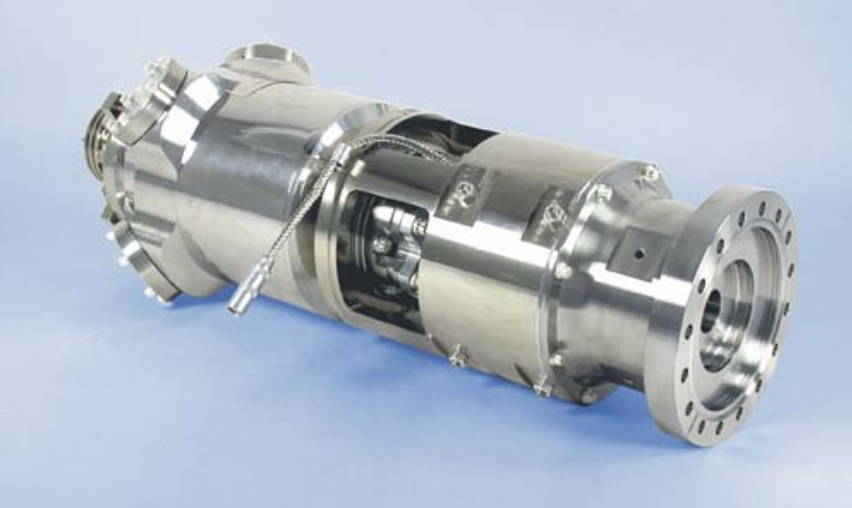
\includegraphics[width=\columnwidth]{figures/ElectronGunEGH6002.png}
 \caption{Photo of a commercially available electron gun from Kimball Physics~\cite{KimballPhysics}. The model EGH-6002 electron gun has the following specifications. Beam energy: 1~keV to 50~keV (adjustable), Beam current: 10~nA to 100 $\mu$A (adjustable), spot-size: 0.5~mm to 100~mm (adjustable with built-in optics), design working distance: 50~mm to 1000~mm. (Not entirely necessary for paper)}
 \label{fig:ElectronGun}
\end{figure}

\subsection{Detectors}
\label{sec:detectors}
Lithium drifted silicon detectors (SiLi) are commonly used in EDX and other X-ray spectroscopy techniques for the range of 1~keV to tens of keV. The more recently developed silicon drift detectors (SDD), however, are becoming much more prevalent because of they are capable of higher count rates and are available with compact thermoelectric that do no require liquid nitrogen. Examples of compact detectors from Amptek \cite{Amptek} are shown in figure \ref{fig:AmptekDetectors}.

\begin{figure}[!h]
 \centering
  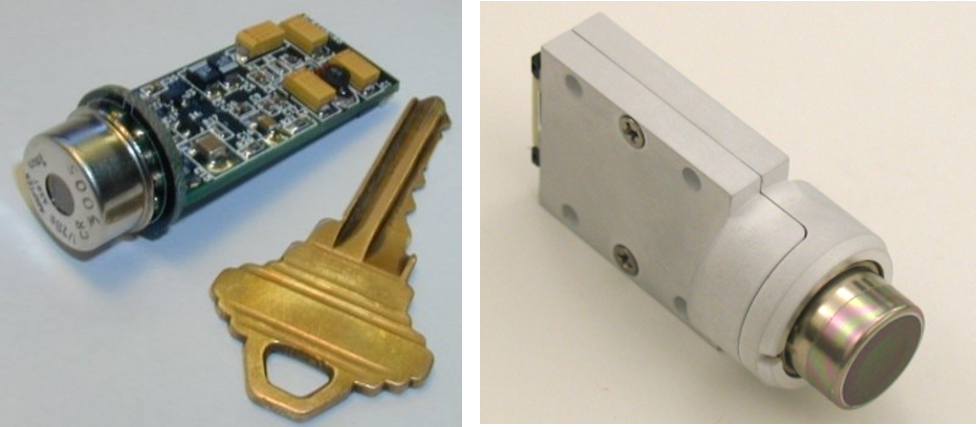
\includegraphics[width=\columnwidth]{figures/SDDPhoto_DoubleCol.pdf}
 \caption{Photos of silicon drift detectors from Amptek with attached pre-amplifier and packaging. Images reproduced from Amptek website \cite{Amptek}.}
 \label{fig:AmptekDetectors}
\end{figure}

SiLi and SDD detectors require the detection element to be hermetically sealed. As a result, the thickness and composition of the X-ray window covering the silicon detector element affects the detection efficiency. Historically, detectors have used beryllium windows making detection of the low energy X-rays from low-Z elements difficult or impossible to measure. Advances in detector window materials however have made detection of these low-Z elements possible.  For example, aluminum coated silicon nitride windows (Si$_3$N$_4$) are now available with favorable characteristics for detecting elements as low-Z as Be, Li, B, C, O, etc.  The window attenuation of K-shell emission from low-Z elements are shown in figure~\ref{fig:DetectorEff} for Amptek C-series (Si$_3$N$_4$) windows and common beryllium windows. These C-series and similar windows are highly advantageous because they now make it possible to study common low-Z coating on tokamak PFCs with EDX.

\begin{figure}[!h]
 \centering
  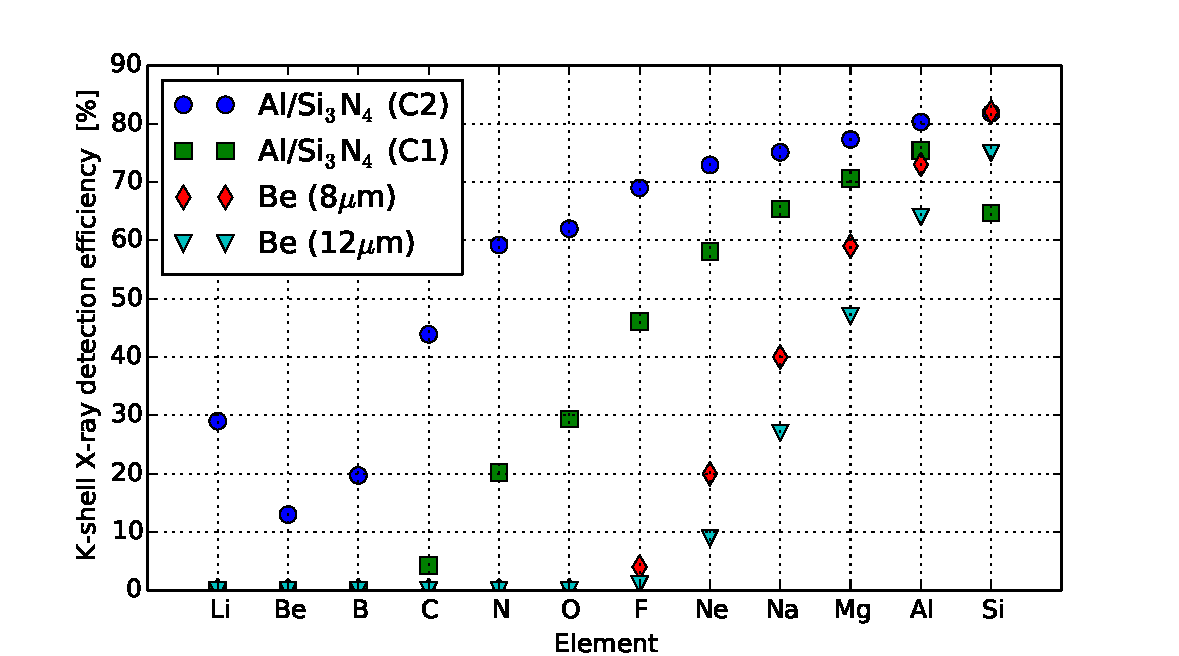
\includegraphics[width=\columnwidth]{figures/KShellDetectorEfficiency.pdf}
 \caption{X-ray windows covering detectors limits low energy X-Ray detection in silicon drift detectors. Detection efficiency for K-shell X-rays are shown for low-Z elements. Beryllium (Be) windows are compared to new window `C-series' windows from Amptek \cite{Amptek}. }
 \label{fig:DetectorEff}
\end{figure}


\subsection{Detection geometry}
\label{sec:DetectionGeometry}

Since the X-rays of interest typically have mean free paths of less than 100~$\mu$m, a line-of-sight path is required between the beam target and detector. This can be achieved by two methods: 1) an array of fixed detectors that are located outside of the plasma region that are distributed poloidally to provide full coverage of target locations or 2) a retractable detector on a robotic arm that maintains close proximity to the beam target. The choice between both of these options is based on the beam current and the corresponding X-ray intensity and the mechanical engineering constraints of the detection hardware. 

The detector must be protected from backscattered electrons and Auger electrons as well as the X-rays that they produce when interacting with surfaces far from the target.  To remove the extraneous X-rays the detectors must have a collimator (e.g. a lead tube) that tracks the position of the beam target location. This can be accomplished with a remotely operated positioning device with 2 degrees of freedom. To prevent backscattered and Auger electrons from reaching the detector, the collimator in combination with electron deflecting permanent magnets can be used. This detector will require some engineering effort but is certainly achievable with technology from modern industrial robotics.

\section{Applications in Alcator C-Mod}

The implementation of in-situ EDX will provide diagnostic capabilities for the affects of many different PMI phenomena. This section focuses on three distinct types of measurements that can be applied to important PMI in Alcator C-Mod: Quantification of boron in surfaces layers due to boronization and subsequent plasma exposure (section~\ref{sec:ApplicationsBoron}), quantification of high-Z transport and migration (section~\ref{sec:ApplicationsTungsten}), and implemenation of depth markers to study bulk PFC material erosion (section~\ref{sec:ApplicationsMarkers}).
\subsection{Measurement of boron}
\label{sec:ApplicationsBoron}

Boron is regularly deposited on PFCs in C-Mod to prevent high-Z impurities from entering the plasma through the boronization process and is used to improve plasma performance \cite{Boronization}. Boron coatings are also useful for studying PMI because changes in the thickness and distribution and be used to study erosion, deposition, and transport of low-Z materials in the plasma. With modern detectors it is now possible to directly measure the K-shell emission from boron, making EDX analysis of boron a powerful tool for PMI science.

X-ray spectra were simulated using MC X-Ray Lite \cite{MCXRayLite} for various thickness boron layers on a molybdenum substrate. From these spectra, shown in figure~\ref{fig:BoronOnMoSpectrum}, the peaks X-ray peaks from Mo and B are clearly distinguishable and measurable above the bremsstrahlung background.

\begin{figure}[!h]
 \centering
  \includegraphics[width=\columnwidth]{figures/BoronOnMoSpectra.pdf}
 \label{fig:BoronOnMoSpectrum}
 \caption{Simulated X-ray spectra from 10-1000~nm boron films on a molybdenum substrate.}
\end{figure}

The X-ray intensities for the B and Mo lines were also calculated as a function of B thickness using CASINO 2.48 \cite{CASINO} and are shown in figure~\ref{fig:BoronIntensity}. Since B is relatively transparent to X-rays compared to Mo and there is relative small beam energy loss in the B layer, the B lines remain relatively unaffected by B thickness up to $\sim 1 \mu$m while the B-K$_\alpha$ line increases monotonically with B thickness over the relevant range for boronization layers in C-Mod.

\begin{figure}[!h]
 \centering
  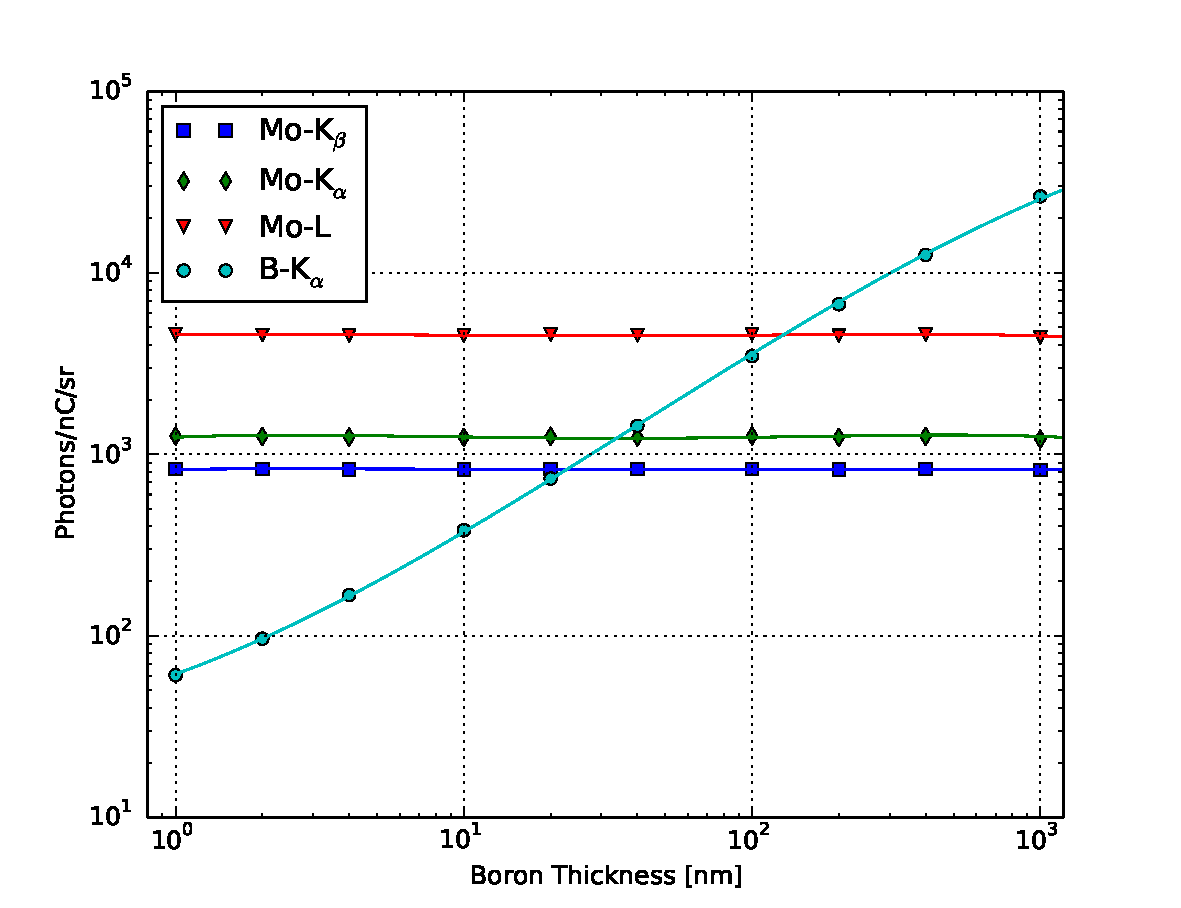
\includegraphics[width=\columnwidth]{figures/cModApplications/Boron_XRayIntensities.pdf}
  %figures/BoronLayerXRayIntensityVsThickness.pdf
 \caption{Calculated intensities for B and Mo X-ray lines for typical thickness of B layers observe on Mo tiles in Alcator C-Mod. B-K$_\alpha$ intensity includes detector X-ray attenuation 20\% attenuation in }
 \label{fig:BoronIntensity}
\end{figure}

\subsection{Measurement of tungsten}
\label{sec:ApplicationsTungsten}
EDX is particularly sensitive to high-Z elements so erosion, deposition and migration of high-Z wall materials can be studied in Alcator C-Mod and other tokamaks by direct measurement. While studies of spatially resolved high-Z material migration have been performed over long timescales (1000-3000 plasma shots) with ex-situ analysis \cite{barnard2011study,Wampler}, in-situ EDX will enable similar measurements after each plasma shot if desired.

% Tungsten_WMoSpectra.pdf
\begin{figure}[!h]
 \centering
  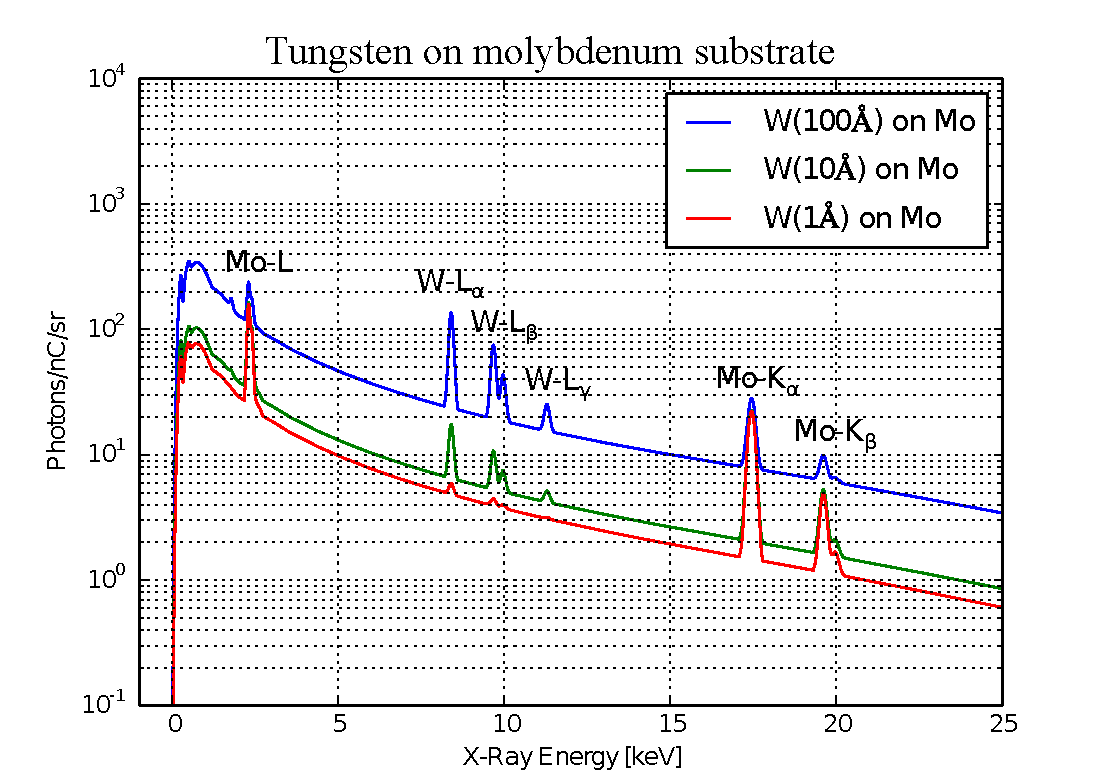
\includegraphics[width=\columnwidth]{figures//cModApplications/Tungsten_WMoSpectra.pdf}
 \caption{}
 \label{fig:Tungsten_WMoSpectra}
\end{figure}

% Tungsten_WMoSpectra.pdf
\begin{figure}[!h]
 \centering
  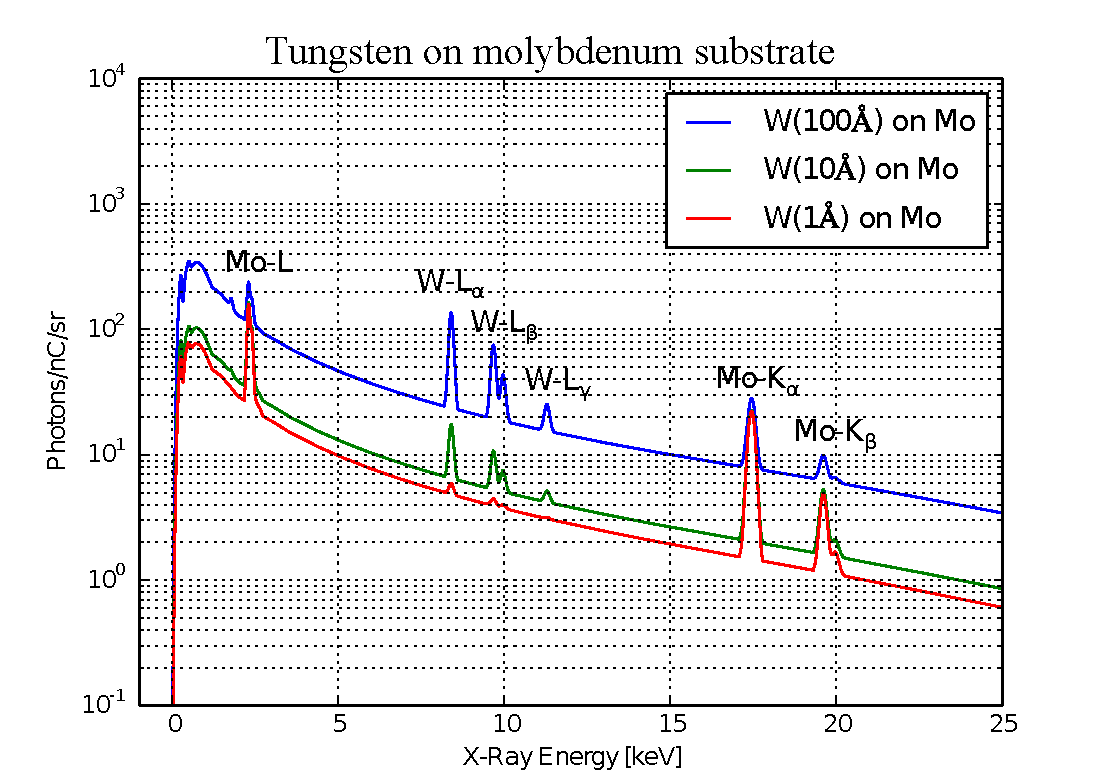
\includegraphics[width=\columnwidth]{figures//cModApplications/Tungsten_WMoSpectra.pdf}
 \caption{}
 \label{fig:Tungsten_WMoSpectra}
\end{figure}


\subsection{Depth-marker analysis}
\label{sec:ApplicationsMarkers}

Implanted depth markers can be used to measure net erosion and deposition of PFC surfaces where the surface as has the same composition as the bulk of the material. To accomplish this, a layer of dissimilar material can be inserted at a well defined depth below a material surface through ion implantation or by a series of deposition processes. Implementation of such markers have been successfully used to in PFCs in Alcator C-Mod and were analyzed using ex-situ Rutherford Backscattering Spectroscopy (RBS) before installation and after removal the tokamak \cite{Wampler}. With in-situ EDX, similar measurements can be made without a vacuum break, after every plasma shot if necessary. 

With EDX, the depth marker performs a somewhat different function than with RBS. The marker will emit characteristic X-rays that are distinguishable from the bulk and the surface material. If the marker is sufficiently thick ($\sim1\;\mu$m), the marker will also suppress the X-ray emission from the bulk of the PFC, allowing the majority of the X-ray to originate in the surface, thus providing greater dynamic range. With these two effects, when the surface above the depth marker is eroded, the intensity of the X-rays from the marker will increase from the reduced attenuation while the emission from the surface will decrease. 

%As a practical c 
% thickness due the effect of surface thickness on X-ray attenuation and average beam energy loss before reaching the depth of the marker. 

The X-ray intensity from the marker and its sensitivity to changes in thickness depend strongly on the X-ray energy, X-ray attenuation in the target material, and the relative X-ray intensity from the bulk of the target material. For maximum sensitivity, the marker material and depth should be optimized to make use of these effects. The marker should be deep enough that a moderate amount of X-ray attenuation and beam energy loss occurs so that both effects contribute to the sensitivity of the measurement to surface changes. This is addressed by placing the marker at a depth that is less than but comparable to the mean free path of the X-rays it produces. The marker and/or the surface X-rays must also produce enough X-rays to compete with emission from the bulk material, otherwise it will be difficult to resolve the marker's X-rays in a spectrum dominated by the bulk material. This can be addressed by using marker with as large an areal density as possible and by using an element that has a higher X-ray emission cross section than the bulk of the material.



% Boron_XRayIntensities.pdf
\begin{figure}[!h]
 \centering
  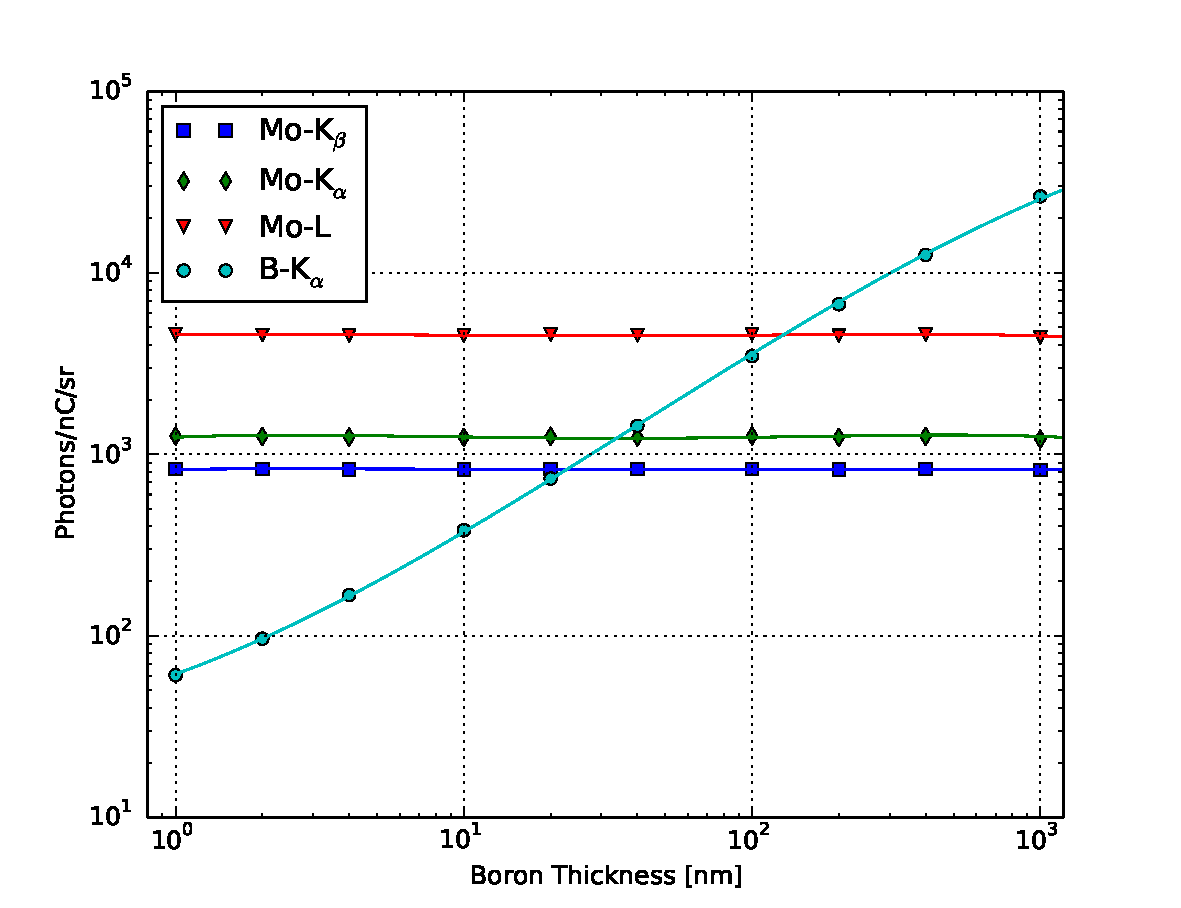
\includegraphics[width=\columnwidth]{figures/cModApplications/Boron_XRayIntensities.pdf}
 \caption{}
 \label{fig:Boron_XRayIntensities}
\end{figure}


% BoronOnMoSpectra.pdf
\begin{figure}[!h]
 \centering
  \includegraphics[width=\columnwidth]{figures//cModApplications/BoronOnMoSpectra.pdf}
 \caption{}
 \label{fig:BoronOnMoSpectra}
\end{figure}



% CrMarker_Spectra.pdf
\begin{figure}[!h]
 \centering
  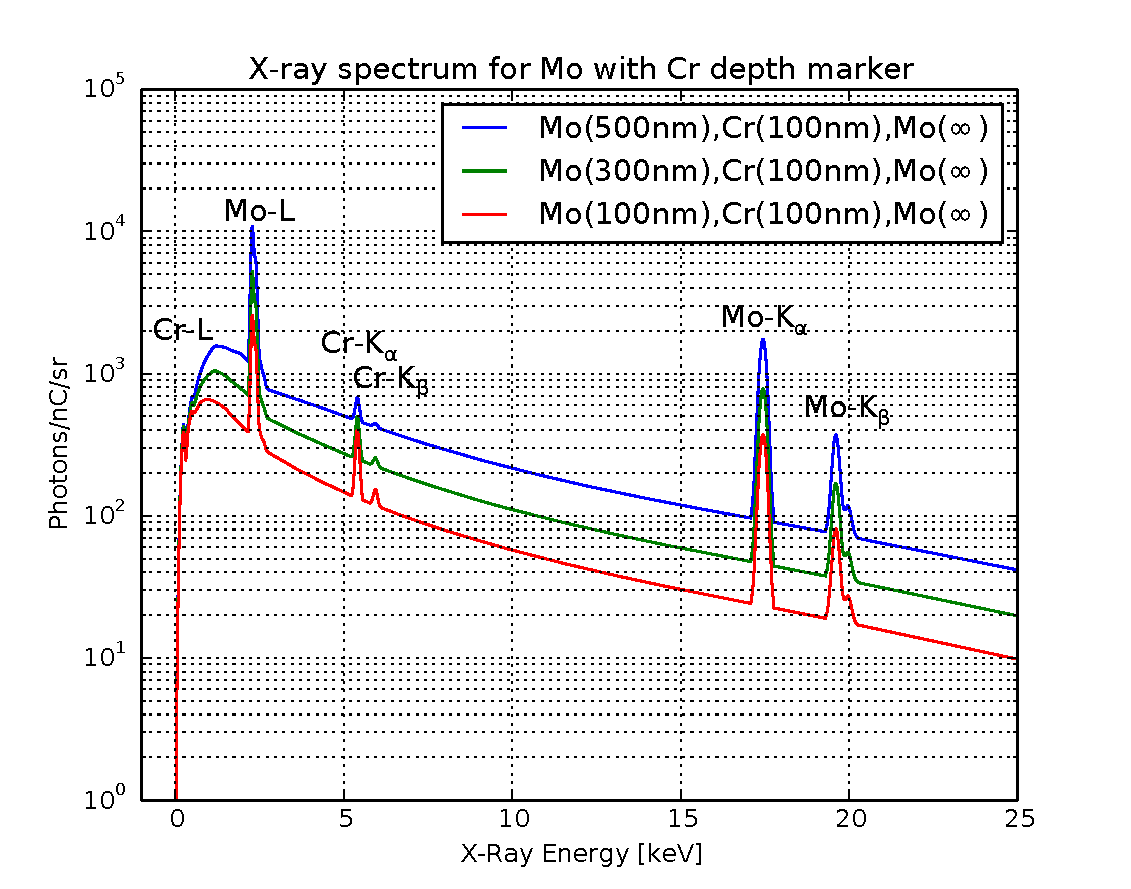
\includegraphics[width=\columnwidth]{figures//cModApplications/CrMarker_Spectra.pdf}
 \caption{}
 \label{fig:CrMarker_Spectra}
\end{figure}

% CrMarker_IntensityLines.pdf
% CrMarker_NormalizeLines.pdf
\begin{figure}[!h]
 \centering
  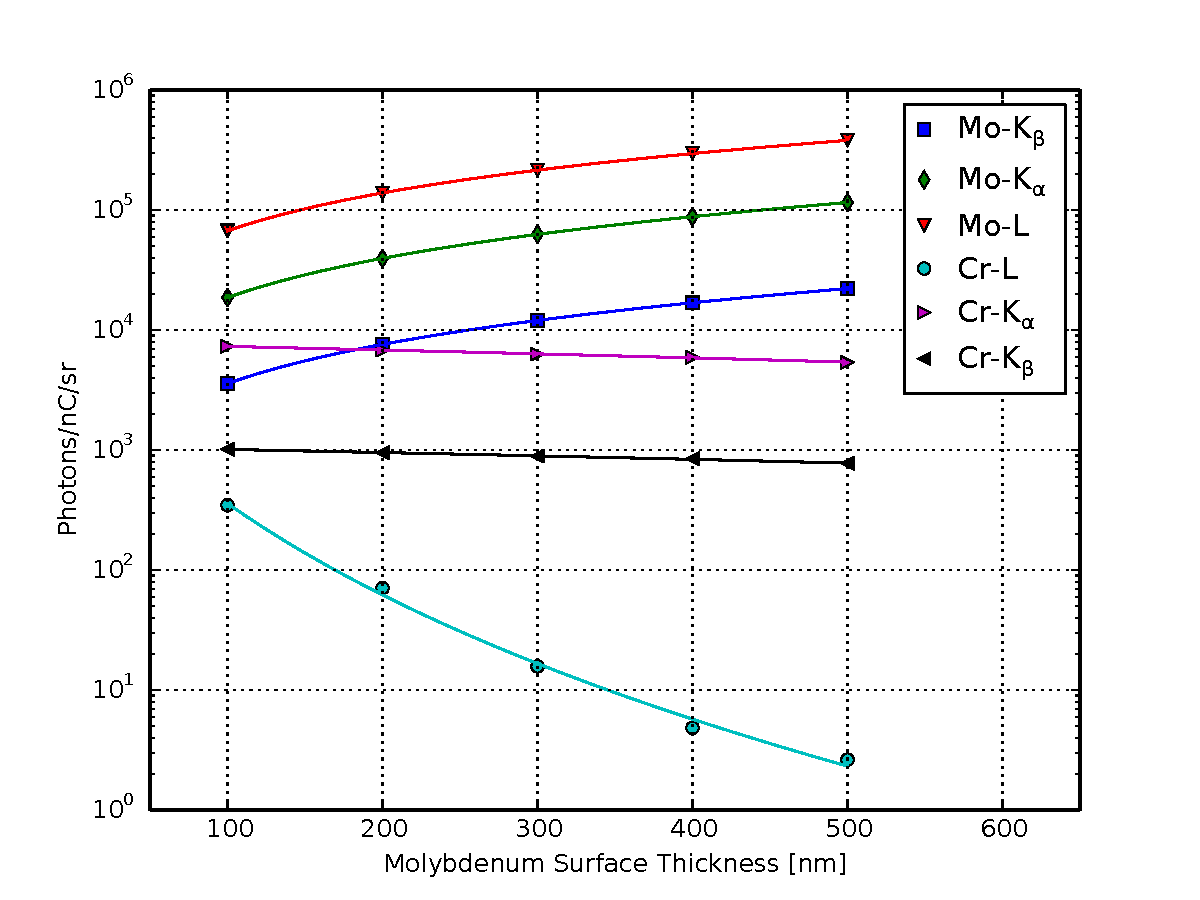
\includegraphics[width=\columnwidth]{figures//cModApplications/CrMarker_IntensityLines.pdf}
 \caption{}
 \label{fig:CrMarker_IntensityLines}
\end{figure}



\bibliographystyle{plain}
\bibliography{ElectronBeamAIMS.bib}
 
\end{document}
